\chapter{\IfLanguageName{dutch}{Opstellen ELK}{Opstellen ELK}}%
\label{ch:Opstellen ELK}
In dit hoofdstuk zal worden gekeken hoe er toegang tot ELK kan worden verleend aan MFPOSS en welke voorbereidingen we hiervoor moeten treffen. Het is niet de bedoeling ELK op de mainframe te installeren, aangezien Colruyt Group Services al ELK buiten de mainframe gebruikt en een team heeft dat het beheert.

\section{Opstellen ELK voor MFPOSS}
Het doel van dit onderzoek is om een prototype van een ELK-dashboard te kunnen leveren aan MFPOSS om te beoordelen of het aan de MoSCoW-eisen voldoet. Om dit te bereiken, moet eerst een contactpersoon worden gevonden bij ELK om te verkennen welke mogelijkheden er zijn om onze data naar ELK te sturen. Het eerste contact met ELK was met Anusha, zij is een medewerker in het OPMONTOOLS-team dat ELK beheert. Vanaf dit punt zullen ze worden aangeduid als het ELK-team. Voordat we doorgaan met het onderzoek, is het belangrijk om te weten of er mogelijkheden zijn om de SYSLOGS naar het ELK-team te sturen. Na een vergadering met Dieter en daarna met Anusha is snel geconcludeerd dat we de gegevens periodiek over TCP/IP kunnen verzenden. Er zijn vermoedens dat Filebeat hiervoor misschien ook kan worden gebruikt, indien nodig. Het besluit om gegevens te verzenden, moet worden genomen voordat ELK wordt opgezet, om onnodig werk te voorkomen. Zodra is besloten dat er een grote kans is om de logs succesvol naar ELK te kunnen sturen, is er een aanvraag ingediend om toegang te krijgen tot ELK. Deze aanvraag is ingediend via ServiceNow. Een verantwoordelijke van het ELK-team zal die aanvraag oppakken en ons verder helpen. Anusha heeft ook gemeld dat als er geen problemen zijn, we binnen tien dagen een integratie kunnen verwachten.


\begin{figure}[h]
    \centering
    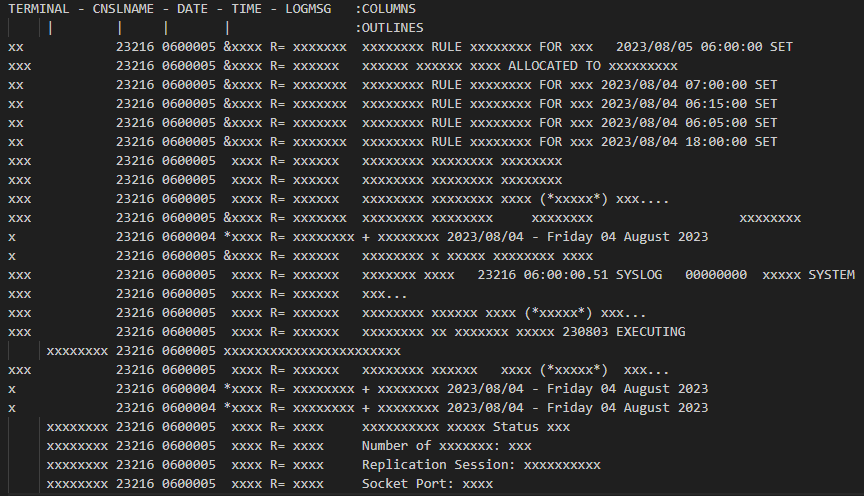
\includegraphics[width=1\linewidth]{bachproef/graphics/Voorbeeld_Syslog.png}
    \caption{Een voorbeeld van een SYSLOG met placeholdergegevens}
    \label{fig:Een voorbeeld van een SYSLOG met placeholdergegevens}
\end{figure}

Dit tekstbestand is per e-mail naar de verantwoordelijken voor de ELK-integratie van MFPOSS gestuurd. Daarbij is ook uitgelegd hoe het voorbeeld is opgebouwd. De eerste regel bevat alle kolomnamen. Daaronder staan regels die het begin van een nieuwe kolom vertegenwoordigen. Vanaf regel drie begint de log zelf. Nu de verantwoordelijken het bestand hebben ontvangen, kunnen ze doorgaan met het opzetten van ELK. Ze hadden ook details nodig over enkele velden, zoals hoe de datum is opgebouwd uit twee tekens voor het jaar en drie tekens voor de dag van het jaar.

\subsection{Mockup}
Nadat een voorbeeld is verzonden, beschikken de verantwoordelijken over alle benodigde informatie om de ELK-integratie voor MFPOSS uit te voeren. Er volgden ook nog enkele vergaderingen waarin het ELK-team details wilde bespreken en bevestigen. Nu de ELK-integratie volop in gang is, kunnen we gelijktijdig beginnen met het ontwerpen van een mock-up voor het dashboard. Dit is het onderwerp van dit hoofdstuk. Op basis van de verwachtingen kunnen we concluderen dat MFPOSS een dashboard nodig heeft waarmee de volgende taken kunnen worden uitgevoerd via panelen:

1. Het bekijken van bepaalde logs.
2. Het detecteren van afwijkingen om te zien of er opvallende gebeurtenissen zijn opgetreden.
3. Mogelijk is er behoefte aan een plek voor documentatie.
4. Een grafiek met interessante gegevens, zoals de meest voorkomende logboekmelding.

\subsubsection{Probleem één}
Tijdens een van de vergaderingen met het ELK-team werd gevraagd naar afwijkingdetectie en wat de mogelijkheden waren om dit in een dashboard te integreren. Het blijkt dat de ELK-stack van Colruyt Group op dat moment nog geen afwijkingdetectie ondersteunt. Dit is een tekortkoming voor MFPOSS, maar het is geen reden om het onderzoek vroegtijdig te stoppen. Met deze nieuwe informatie kunnen we punt twee schrappen. Dit geeft ons ruimte om een andere grafiek toe te voegen.

\begin{figure}[h]
    \centering
    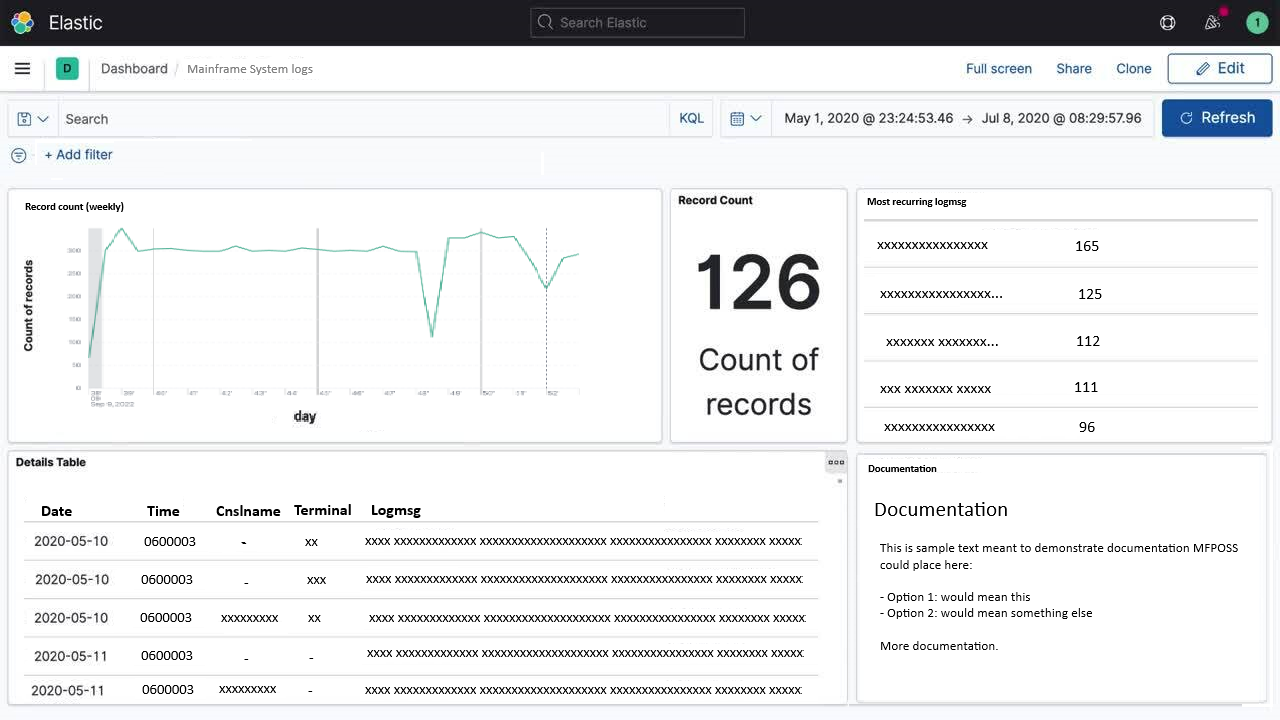
\includegraphics[width=1\linewidth]{bachproef//graphics/Dashboard_mockup.png}
    \caption{De mock-up voor het ELK-dashboard van MFPOSS}
    \label{fig: De mock-up voor het ELK-dashboard van MFPOSS}
\end{figure}

Figuur 4.3 is een mock-up van een dashboard dat mogelijk wordt verwacht. Het dashboard bestaat naast de Elastic-header uit vijf panelen. Er wordt hier natuurlijk gewerkt met fictieve gegevens die zo goed mogelijk echte gegevens proberen te representeren. Laten we kort de panelen bespreken. Het paneel op de eerste rij is een paneel met een lijngrafiek. Dit dient om te laten zien hoeveel regels de logs bevatten gedurende de afgelopen zeven dagen. Daarnaast is er een kleiner paneel dat snel het aantal regels weergeeft dat vandaag is ontvangen. Dit is handig om gemakkelijker te vergelijken met voorgaande dagen op de grafiek. Paneel drie is een lijst met de meest voorkomende regels. Een ervaren medewerker zou hier hopelijk al afwijkingen kunnen opmerken, aangezien afwijkingdetectie niet wordt gebruikt binnen Colruyt Group. Het tweede rij aan panelen bevat er twee: links de meest recente logs die ELK heeft ontvangen, en rechts een kader dat dient voor documentatie, tips of notities. Dit dashboard bevat al een groot deel van wat MFPOSS snel wil zien. Maar als men dieper in de gegevens wil kijken, is er ook de mogelijkheid om velden te doorzoeken en te visualiseren met behulp van de zoekbalk bovenaan.


